%
% automorphismus.tex
%
% (c) 2021 Prof Dr Andreas Müller, OST Ostschweizer Fachhochschule
%
\begin{frame}[t]
\setlength{\abovedisplayskip}{4pt}
\setlength{\belowdisplayskip}{4pt}
\frametitle{Galois-Gruppe}
\vspace{-20pt}
\begin{columns}[t,onlytextwidth]
\begin{column}{0.40\textwidth}
\begin{center}
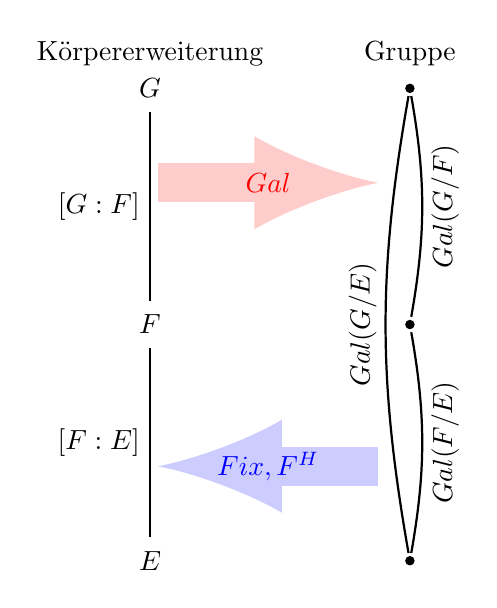
\begin{tikzpicture}[>=latex,thick]
\def\s{3.0}
\begin{scope}[xshift=-1.5cm]
\node at (0,{\s+0.1}) [above] {Körpererweiterung\strut};
\node at (0,{\s}) {$G$};
\draw[shorten >= 0.3cm,shorten <= 0.3cm] (0,{-\s}) -- (0,0);
\draw[shorten >= 0.3cm,shorten <= 0.3cm] (0,{\s}) -- (0,0);
\node at (0,{-0.5*\s}) [left] {$[F:E]$};
\node at (0,{0.5*\s}) [left] {$[G:F]$};
\node at (0,0) {$F$};
\node at (0,{-\s}) {$E$};
\end{scope}
\uncover<3->{
\begin{scope}[xshift=1.8cm]
\node at (0,{\s+0.1}) [above] {Gruppe\strut};
\fill (0,{-\s}) circle[radius=0.06];
\fill (0,0) circle[radius=0.06];
\fill (0,{\s}) circle[radius=0.06];
\draw[shorten >= 0.1cm,shorten <= 0.1cm]
	(0,{-\s}) to[out=100,in=-100] (0,{\s});
\draw[shorten >= 0.1cm,shorten <= 0.1cm]
	(0,{-\s}) to[out=80,in=-80] (0,0);
\draw[shorten >= 0.1cm,shorten <= 0.1cm]
	(0,0) to[out=80,in=-80] (0,{\s});
\node at (-0.6,0) [rotate=90] {$\operatorname{Gal}(G/E)$};
\node at (0.45,{0.5*\s}) [rotate=90] {$\operatorname{Gal}(G/F)$};
\node at (0.45,{-0.5*\s}) [rotate=90] {$\operatorname{Gal}(F/E)$};
\end{scope}
\draw[->,color=red!20,line width=14pt] (-1.4,{0.6*\s}) -- (1.4,{0.6*\s});
\node[color=red] at (0,{0.6*\s}) {$\operatorname{Gal}$};
}
\uncover<4->{
\draw[<-,color=blue!20,line width=14pt] (-1.4,{-0.6*\s}) -- (1.4,{-0.6*\s});
\node[color=blue] at (0,{-0.6*\s}) {$\operatorname{Fix}, F^H$};
}
\end{tikzpicture}
\end{center}
\end{column}
\begin{column}{0.56\textwidth}
\uncover<2->{%
\begin{block}{Automorphismus}
\vspace{-10pt}
\[
\operatorname{Aut}(F)
=
\left\{
f\colon F\to F
\left|
\begin{aligned}
f(x+y)&=f(x)+f(y)\\
f(xy)&=f(x)f(y)
\end{aligned}
\right.
\right\}
\]
\end{block}}
\vspace{-10pt}
\uncover<3->{%
\begin{block}{Galois-Gruppe}
Automorphismen, die $E$ festlassen
\[
{\color{red}
\operatorname{Gal}(F/E)
}
=
\left\{
\varphi\in\operatorname{Aut}(F)\;|\; \varphi(x)=x\forall x\in E
\right\}
\]
\end{block}}
\vspace{-10pt}
\uncover<4->{%
\begin{block}{Fixkörper}
$H\subset \operatorname{Aut}(F)$:
\begin{align*}
{\color{blue}F^H}
&=
\{x\in F\;|\; hx = x\forall h\in H\}
=\operatorname{Fix}(H)
\end{align*}
\end{block}}
\vspace{-13pt}
\uncover<5->{%
\begin{block}{Beispiel}
\begin{itemize}
\item<6->
\(
\operatorname{Gal}(\mathbb{C}/\mathbb{R})
=
\{
\operatorname{id}_{\mathbb{C}},
\operatorname{conj}\colon z\mapsto\overline{z}
\}
\)
\item<7->
\(
\mathbb{C}^{\operatorname{conj}}
=
\mathbb{R}
\)
\end{itemize}
\end{block}}
\end{column}
\end{columns}
\end{frame}
